
\section{Introduction}
\label{sec:introduction}

\eat{
% OLD VERSION
\begin{figure}
    \centering
  %  \includegraphics[trim=0 0 0 0,clip, width=\textwidth]{figures/NuerIps 24 - Fig 1 - Teaser PNAS Style - Bigger.pdf}
  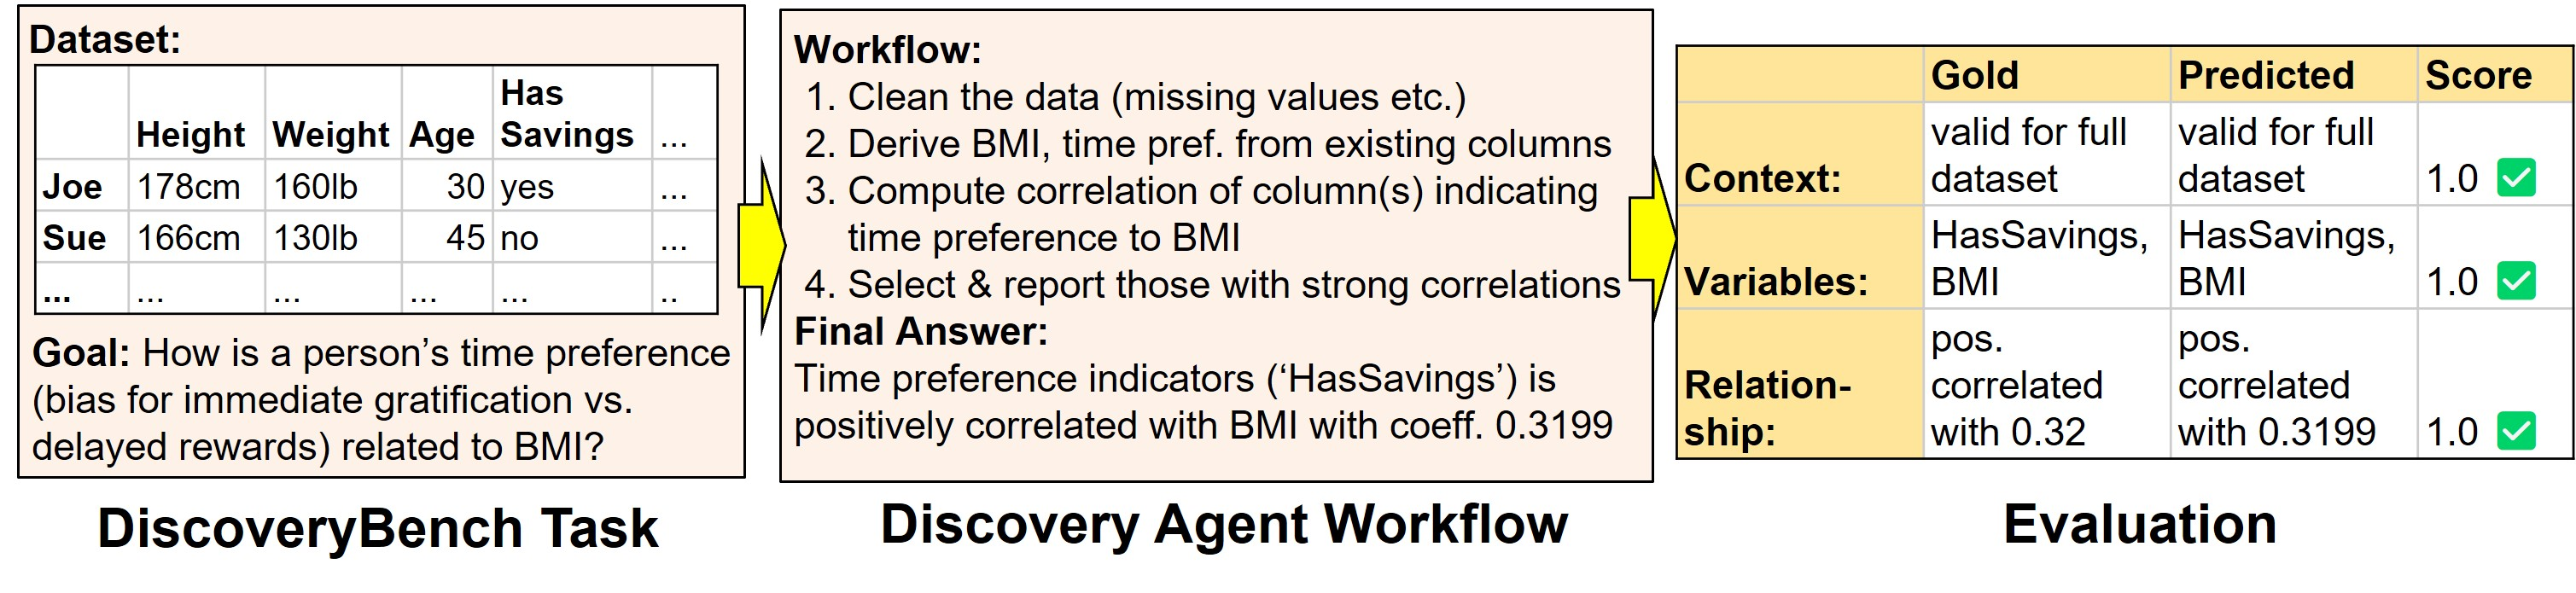
\includegraphics[width=1\columnwidth]{figures/Figure1.jpg}
%    \caption{WIP Teaser Figure, needs iteration on content and layout}
    \caption{Each DiscoveryBench task consists of a goal and dataset(s) (left). Solving the task requires both statistical analysis and semantic reasoning, e.g., mapping goal terms to column names (center). A faceted evaluation allows open-ended final answers to be rigorously evaluated (right).}
    \label{fig:teaser}
\end{figure}
}

% Why is automated discovery important? Why data-driven discovery? (use position paper points).
Knowledge discovery via the scientific process 
has been a catalyst for human progress for centuries
but has, thus far, been a predominantly manual pursuit \citep{glass2008brief}. 
Recent breakthroughs in capabilities of large language models (LLMs) to reason and interface with the world using code \citep{chen2021evaluating, roziere2023code}, external tools \citep{schick2024toolformer}, and interactive agents \citep{yao2023react, majumder2023clin}, however, now suggest the possibility of realizing a discovery system that is fully autonomous.
Indeed, recent works \citep{majumder2024data} provide initial evidence for this paradigm within the setting of \emph{data-driven discovery}, where both search and verification of hypotheses may be carried out using a dataset alone (i.e., 
after physical experiments and data collection\footnote{
    In practice, experiments and analysis are interleaved, not sequential. Our concern
    in this work, however, is systematically studying the data analysis part of the (interleaved) pipeline.
    }),
% without the need for physical experiments or additional data collection),
but the extent of this ability remains unclear. 
We, therefore, aim to systematically evaluate the following question: 

{\centering
    \emph{How good are current state-of-the-art LLMs at automated data-driven discovery?}\par
}

\eat{
To answer this question, several challenges must be addressed. 
Data-driven discovery in the wild (real-world) is often noisy and may take diverse forms across domains and subject areas. This makes the formalization of the discovery task challenging from an algorithmic perspective, which, in turn, also makes it difficult to build a robust evaluation framework to measure progress. Furthermore, the lack of standardization and reproducibility in several domains renders the automated, large-scale collection of real-world trajectories for hypothesis search and verification extremely difficult.
% However, no systematic study exists. Prior works insufficient for various reasons. Closest work is QRData. What are some challenges with doing systematic study? (real-world data not easily available, discovery process is often not well-defined making it hard to construct this as a task and measure performance)


We address each of these challenges and present \discoverybench{}---a novel benchmark for evaluating automated data-driven discovery using LLMs. \dhruv{TBA: describe the task using the to-be-added new figure (@bodhi).} \ashish{an example would be super helpful to ground the reader's thinking!}

Our contributions are as follows: \textbf{(a)} \discoverybench{} is the first comprehensive \ashish{unclear in what way is the benchmark `comprehensive' or what would make such a benchmark comprehensive} benchmark to formalize the multi-step process of data-driven hypothesis search and verification. \textbf{(b)} We manually extract 262 \ashish{abstract says 264} discovery tasks from over XXXX published papers across 6 diverse domains to provide wide coverage of real-world discovery workflows. \textbf{(c)} Using our novel task formalism, we further provide 903 synthetic tasks across 48 domains generated using LLMs to mimic the real-world discovery process. The synthetic benchmark allows us to conduct controlled model evaluations by varying task difficulty and also serves as a resource to improve models via fine-tuning. \textbf{(d)} We conduct a comprehensive evaluation across state-of-the-art reasoning frameworks \ashish{not sure if `framework' is the right word, if you are referring to ReAct, Reflexion, etc.; also, there are non-LLM based reasoning frameworks too. Could instead simplify and combine into `state-of-the-art LLM-based reasoning methods'. Same note for the abstract.} and LLMs on \discoverybench{} and find that performance peaks at $16\%$, demonstrating the challenging nature of our task.

\ashish{a mention of `agents' is missing. would be good to find a way to connect with agents / agent-based frameworks.}
}

\begin{figure}
    \centering
  %  \includegraphics[trim=0 0 0 0,clip, width=\textwidth]{figures/NuerIps 24 - Fig 1 - Teaser PNAS Style - Bigger.pdf}
  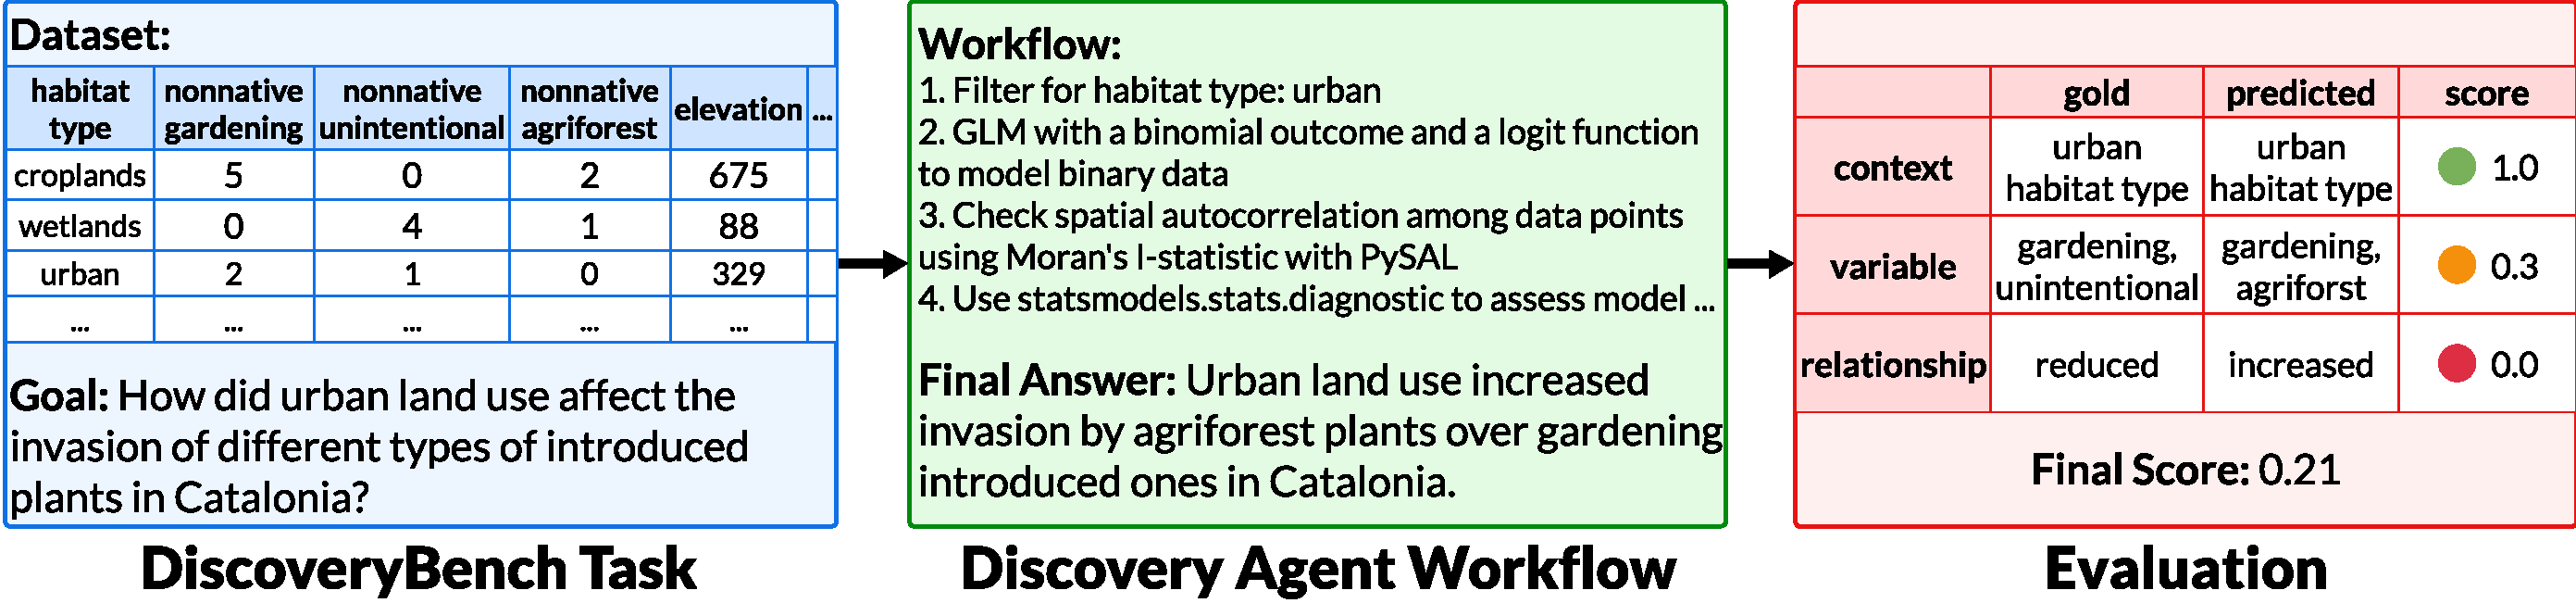
\includegraphics[width=1\columnwidth]{figures/Fig1_Workflow_Example_Climate1.pdf}
%    \caption{WIP Teaser Figure, needs iteration on content and layout}
 \caption{\small Each \discoverybench{} task consists of a goal and dataset(s) (left). Solving the task requires both statistical analysis and scientific semantic reasoning, e.g., deciding which analysis is appropriate for the domain, and mapping goal terms to column names (center). A faceted evaluation allows open-ended final answers to be rigorously evaluated (right).}
%     \caption{WIP: Peter's figure workflow with alternative example. Selected this to address Ashish's concern on time-preference being confusing, differentiate from ML datasets on workflow and to address a more relevant topic: climate. If this is too complicated, we can add Peter's example in this format as well.}
    \label{fig:teaser}
\end{figure}

Answering this question is hard, as data-driven discovery in the wild (real-world) is
diverse across domains and subject areas, which in turn makes it difficult to build
a robust evaluation framework to measure progress.
We address this using a pragmatic formalization of data-driven discovery, namely
the search for a {\it relationship} that may hold between {\it variables} in a {\it context},
where (importantly) the description of those facets may not be in the language of the
dataset. A data-driven discovery task then has one of these components missing, e.g., ``How
did urban land use affect the invasion of introduced plants in Catalonia?".
Importantly, this formalization allows for systematic,
reproducible evaluation over a wide variety of real-world problems, by leveraging these facets (Fig~\ref{fig:teaser}, right).

Unlike prior datasets for statistical analysis \cite{liu2024llms} or AutoML \cite{Zhang2023AutoMLGPTAM, Gijsbers2022AMLBAA}, 
\discoverybench{} tasks
also require scientific semantic reasoning, for instance, deciding which of the many possible
analysis techniques are appropriate for the domain (e.g., spatial autocorrelation for
plant invasion, Fig~\ref{fig:teaser} center), how to clean and/or normalize the data, 
and how to map goal terms to dataset terms (e.g., ``land use'' to ``habitat type''). Task
solutions typically requires a multistep workflow (Fig~\ref{fig:teaser}, center). 
In this way, \discoverybench{} is the first
large-scale dataset to address the broader data-driven discovery pipeline, not just
the statistical analysis component, and explore LLMs' capacity for this.

Given this framework, we created \discoverybench{} by manually extracting 264 discovery tasks, i.e., goal + dataset(s), from over 20 published papers, as well as creating real-world discovery workflows
that solve each task. We additionally provide 903 synthetic tasks across 48
domains generated using LLMs to mimic the real-world discovery process. The synthetic
benchmark allows us to conduct controlled model evaluations by varying task difficulty.
% and also
% serves as a resource to improve models via fine-tuning.
Our contributions are thus:
\begin{ite}
  \item \discoverybench, the first comprehensive benchmark to formalize 
    the multi-step process of data-driven hypothesis search and verification,
    covering many real-world discovery tasks plus additional synthetic tasks.
  \item A pragmatic formalism for data-driven discovery, flexible enough to
    characterize many real-world tasks while constrained enough to allow
    for rigorous, reproducible evaluation.
  \item A comprehensive evaluation across state-of-the-art LLM-based reasoning methods (``discovery agents'').
    We find performance peaks at 25\%, demonstrating the challenging nature of our task.
\end{ite}
These suggest that \discoverybench{} may be a valuable resource for helping make progress
on autonomous, data-driven discovery.


% \ashish{Unless the Related Work section will be very large, it feels valuable to place it right after the intro. I personally like it that way, but importantly for this paper, people would want to know what else is out there, what's novel here, why existing data science benchmarks don't suffice, etc. In other words, if we can (somewhat brielfy) situate this work in the context of what exists, people will appreciate the technical content more (e.g., the notation they are about to read in Preliminaries).}
